\subsection*{Solution to Fall 2014, \#1}
\label{F14Q1}

\subsubsection*{Solution to $1a$}

The system of ODEs represents a predator-prey system. For the species represented by $x$, the $2x$ term represents growth for the species, the $-x^2$ term represents a decay of the species, and the $-xy$ term represents competition between species $x$ and $y$. For the species represented by $y$, the $y$ term represents growth for the species, and the $-xy$ term represents competition between species $x$ and $y$.

\subsubsection*{Solution to $2a$}

Setting $\dot{x}$ and $\dot{y}$ equal to 0 yields the following fixed points: $(0,0), (1,1), (2,0)$. Define $F(x,y) := (2x-x^2-xy, y-xy)$, and compute the Jacobian
$$ J[F](x,y) = \pmat{2-2x-y}{-x}{-y}{1-x} $$
Then, we compute eigenvalues and eigenvectors:
$$ J[F](0,0) = \pmat{2}{0}{0}{1} \quad \implies \quad \evev{2}{1}{1}{0}{0}{1}$$
$$ J[F](1,1) = \pmat{-1}{-1}{-1}{0}  \implies\evev{\frac{-1+\sqrt{5}}{2}}{\frac{-1-\sqrt{5}}{2}}{1-\sqrt{5}}{2}{1+\sqrt{5}}{2} $$
$$ J[F](2,0) = \pmat{-2}{-2}{0}{-1}\quad \implies \quad \evev{-2}{-1}{1}{0}{-2}{1} $$
Below is a plot of the phase plane.

\begin{center}
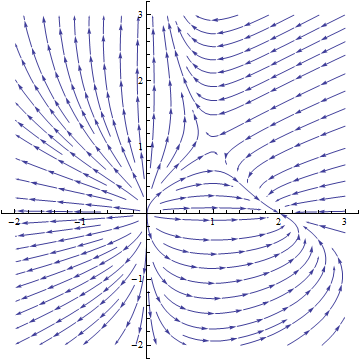
\includegraphics[scale=0.75]{./_Figures/f141_ppp.png}
\end{center}

The nullclines are the contours $2x-x^2-xy=0$ and $y-xy=0$, which are not shown in the plot above.
For large $x, y$, $\dot{x} \approx -x^{2} - xy$ and $\dot{y} \approx -xy$ and hence
$$\frac{dx}{dy} \approx \frac{-x - y}{-y} = 1 + \frac{x}{y}.$$
Therefore
$$\frac{dx}{dy} - \frac{x}{y} - 1 = 0.$$
Dividing both sides by $y$ yields that
$$\frac{d}{dy}\left(\frac{1}{y}x\right) = \frac{1}{y}$$
which gives $x = y\log y + Cy$. Therefore the trajectories look like
$x = y\log y + Cy$ for $x, y$ large.





\subsection*{Solution to Fall 2014, \#2}
\label{F14Q2}

\subsubsection*{Solution to $2a$}

We are looking to find $y$ and $\lambda$ such that
\[
x^2 y'' + x y' + \lambda y = 0, \quad \text{where} \quad y(1) = y(2) = 0
\]
First, observe notice $\lambda \neq 0$. If $\lambda$ were zero, then
\[
x^2 y'' + xy' = 0 \quad \implies \quad y' = \frac{C}{x} \quad \implies \quad y = C \ln(x) + D
\]
for constants $C$ and $D$ However, this solution doesn't satisfy the boundary conditions unless $y \equiv 0$, implying $\lambda = 0$ is not an eigenvalue.

With the ansatz $y = x^n$, observe
\[
x^2 y'' + x y' + \lambda y = n(n-1)x^n + n x^n + \lambda x^n = 0 \quad \implies \quad n^2 = - \lambda
\]
If $\lambda < 0$, then $n = \pm \sqrt{-\lambda}$, and
\[
y= A x^{\sqrt{-\lambda}} + Bx^{-\sqrt{-\lambda}}
\]
The only choice of constants $A$ and $B$ such that $y$ satisfies the boundary conditions is $A = B = 0$, so any choice of $\lambda < 0$ is not an eigenvalue. 						

If $\lambda > 0$, then $n = \pm i \sqrt{\lambda}$, and
\[
x^{\pm i \sqrt{n}} = \cos(\sqrt{\lambda} \ln(x)) \pm i \sin(\sqrt{\lambda} \ln (x))
\]
Hence,
\[
y = A \cos ( \sqrt{\lambda} \ln (x)) + B \sin( \sqrt{\lambda} \ln (x))
\]
In order for $y$ to satisfy the boundary conditions, we get $A=0$ and $\lambda = \left( \frac{k \pi}{\ln 2} \right)^2$ for $k > 1$. Thus it follows the eigenfunctions are
\[
\mu_k(x) = \sin \left( \frac{k \pi \ln x}{\ln 2} \right)
\]
with associated eigenvalue $\lambda_k =  \left( \frac{k \pi}{\ln 2} \right)^2$. \hfill \qed

\subsubsection*{Solution to $2b$}

In order to use our previous work to our advantage, we first show that ODE is a Sturm-Liouville problem. Indeed,
\[
x^2 y'' + xy' + \lambda y = 0 \quad \implies \quad x [ (xy')'] = -\lambda y
\]
which is now in Sturm-Liouville form. Thus, the operator $Ly := x[(xy')']$ is self-adjoint with respect to the weighted inner product $<u,v>_{r(x)} = \int_1^2 u(x)v(x) r(x) \, dx$, where $r(x) = \frac{1}{x}$. This implies that the set of eigenfunctions $\{ \mu_k(x) \}$ for $k > 1$ forms an orthogonal basis. Now, the solution $y$ to
\[
x^2 y'' + x y' + 3y = x \log x \quad \text{where} \quad y(1) = y(2) = 0
\]
can be represented as
\begin{equation}
\label{F14Q2Eq1}
y(x) = \sum_{k=1}^{\infty} a_k \mu_k(x)
\end{equation}
Before solving for $a_k$, observe
\begin{equation}
\label{F14Q2Eq2}
x^2 y'' + x y' + 3y = x \log x \quad \implies \quad (L + 3I) y = x \log x
\end{equation}
where $L$ is defined above and $I$ is the identity operator. Because the eigenfunctions form an orthogonal basis, we may also write
\[
x \log x = \sum_{k=1}^{\infty} f_k \mu_k(x) \quad \text{where} \quad f_k = \dfrac{\int_1^2 \log (x) \mu_k(x) \, dx}{\int_1^2 \mu_k(x)^2 r(x) \, dx}
\]
Now, plugging \eqref{F14Q2Eq1} into \eqref{F14Q2Eq2} yields
\begin{align*}
(L + 3I) \left( \sum_{k=1}^{\infty} a_k \mu_k(x) \right) = \sum_{k=1}^{\infty} f_k \mu_k(x) \quad &\implies \quad \sum_{k=1}^{\infty} a_k (\lambda_k + 3) \mu_k (x) = \sum_{k=1}^{\infty} f_k \mu_k(x) \\
&\implies \quad a_k = \frac{f_k}{\lambda_k + 3}
\end{align*}
Therefore, the solution is
\[
y(x) = \sum_{k=1}^{\infty} \frac{f_k}{\lambda_k+3} \mu_k(x) \quad \text{where} \quad f_k = \dfrac{\int_1^2 \log (x) \mu_k(x) \, dx}{\int_1^2 \mu_k(x)^2 r(x) \, dx}
\]
Note that there are no solutions to the homogeneous version of this ODE. If there were, then $\lambda = 3$ would be an eigenvalue of the ODE in part (a), which is a contradiction to our work above. \hfill \qed


\subsection*{Solution to Fall 2014, \#3}
\label{F14Q3}

\subsubsection*{Solution to $3a$}

We solve this using method of characteristics. Since the PDE is quasilinear, we only need the following three ODEs to solve the PDE:
\begin{align}
\label{f143t} &\dot{t}(s) = 1, \quad t(0) = 0 \\
\label{f143x} &\dot{x}(s) = z(s), \quad x(0) = x_0 \\
\label{f143z} &\dot{z}(s) = 0, \quad z(0) = \cos(x_0)
\end{align}
Solving \eqref{f143t} and \eqref{f143z} yield
$$ t(s) = s, \quad \text{and} \quad z(s) = z(t) = \cos(x_0) $$
respectively. Then, solving for \eqref{f143x} yields
$$ x(s) = x(t) = \cos(x_0) t + x_0 $$
Therefore, $u(x,t) = \cos(x_0)$ where $x = \cos(x_0)t + x_0$. \hfill \qed

\subsubsection*{Solution to $3b$}

First, note that our solution won't be continuous for all time. To see this, consider two characteristics that start at $a$ and $b$, where $a \neq b$ and $\cos(a) \neq \cos(b)$. These two characteristics will intersect when
$$ \cos(a) t + a = \cos(b) t + b \quad \implies \quad t = \frac{b-a}{\cos(a) - \cos(b)} $$
However, this analysis is not entirely accurate. Since the characteristics are straight lines that are not all parallel, we can find $c$ where $a < c < b$ such that the characteristic starting at $c$ will crash into either the characteristic starting at $a$ or $b$ first. At this point, we either (1) stop defining our solution because we want something that's continuous, or (2) apply the Rakine-Hugoniot condition to figure out the shock curve that starts at the crash. Either way, this implies that the characteristics starting at $a$ and $b$ will never crash as long as $a \neq b$ and $\cos(a) \neq \cos(b)$. Hence, we must examine characteristics that start arbitrarily close to each other in order to obtain accurate data about them intersecting.

Letting $b$ tend to $a$ yields $t = 1/\sin(a)$. Hence, if we let $a = \pi/2$, we now know that characteristics that start arbitrarily close to $\pi/2$ will crash close to $t=1$, which is the smallest time for which discontinuities in our solution will occur.

For $t < 1$, our solution is continuous. Furthermore, along the characteristic that starts at $x_0 = 0$, $u(x,t) = 1$. Because of the behavior of cosine, we know that $u(x,t) \leq 1$, which implies $\max_{x \in \R} u(x,t) = 1$. \hfill \qed






\subsection*{Solution to Fall 2014, \#4}
\label{F14Q4}

\subsubsection*{Solution to $4a$}

Let $v \in H^1_0((0,1))$ be an arbitrary test function. Then, integration by parts yields
$$ \int_0^1 \d_x(\beta u_x) v \, dx = \int_0^1 fv \, dx \quad \implies \quad -\int_0^1 \beta u_x v_x \, dx = \int_0^1 fv \, dx $$
which is the weak form. Note that $\beta u_x$ is continuous at $\hat{x}$, so we don't need to split up the integral at $\hat{x}$. Furthermore, because $v$ vanishes at the endpoints, the boundary terms vanish.

\subsubsection*{Solution to $4b$}

We first construct the Green's function for the case where $x_0 < \hat{x}$. For $x \neq x_0$, the ODE boils down to
$$
-\frac{\d}{\d x} \left( \beta(x) G_x(x;x_0) \right) = 0 \quad \implies \quad G(x;x_0) = \left\{
\begin{array}{ll}
a_1 + a_2 x & \text{if} \,\, 0 \leq x < x_0 \\
b_1 + b_2 x & \text{if} \,\, x_0 < x < \hat{x} \\
c_1 + c_2 x & \text{if} \,\, \hat{x} < x \leq 1
\end{array} \right.
$$
where $a_1, a_2, b_1, b_2, c_1, c_2$ are constants. From the conditions of our problem, we have
\begin{align}
\label{f1441} &G(0,x_0) = G(1,x_0) = 0 \quad \implies \quad a_1 = 0, \,\,\, c_1 + c_2 = 0 \\
\label{f1442} &G(\hat{x}^+,x_0) = G(\hat{x}^-,x_0) \quad \implies \quad c_1 + c_2 \hat{x} = b_1 + b_2 \hat{x} \\
\label{f1443} &\beta(\hat{x}^+)G_x(\hat{x}^+,x_0) = \beta(\hat{x}^-)G_x(\hat{x}^-,x_0) \quad \implies \quad 2c_2 = b_2
\end{align}
We also have
$$ \int_{x_0^-}^{x_0^+} -\frac{\d}{\d x} \left( \beta(x) G_x(x,x_0) \right) \, dx = \int_{x_0^-}^{x_0^+} \delta(x-x_0) \, dx = 1 $$
Since $x_0 < \hat{x}$, this implies
\begin{equation}
\label{f1444} G_x(x_0^+,x_0) - G_x(x_0^-, x_0) = -1 \quad \implies \quad b_2 - a_2 = -1
\end{equation}
We also need $G(x,x_0)$ to be continuous at $x=x_0$, so we want
\begin{equation}
\label{f1445} a_2 x_0 = b_1 + b_2 x_0
\end{equation}
Solving \eqref{f1441} through \eqref{f1445} yields the following Green's function for $x_0 < \hat{x}$
$$ G(x,x_0) =
\left\{
\begin{array}{ll}
\left( 1 -\dfrac{2x_0}{\hat{x}+1} \right) x & \text{if} \,\,\, 0 \leq x < x_0 \\ \asep
x_0 - \dfrac{2x_0}{\hat{x}+1} x & \text{if} \,\,\, x_0 < x < \hat{x} \\ \asep
\dfrac{x_0}{\hat{x}+1} (1-x) & \text{if} \,\,\, \hat{x} < x \leq 1
\end{array}
\right. $$
For $x_0 > \hat{x}$, we now have
$$ G(x;x_0) = \left\{
\begin{array}{ll}
a_1 + a_2 x & \text{if} \,\, 0 \leq x < \hat{x} \\
b_1 + b_2 x & \text{if} \,\, \hat{x} < x < x_0 \\
c_1 + c_2 x & \text{if} \,\, x_0 < x \leq 1
\end{array} \right.
$$
with the conditions
\begin{align}
\label{f1446} &G(0,x_0) = G(1,x_0) = 0 \quad \implies \quad a_1 = 0, \,\,\, c_1 + c_2 = 0 \\
\label{f1447} &G(\hat{x}^+,x_0) = G(\hat{x}^-,x_0) \quad \implies \quad b_1 + b_2 \hat{x} = a_1 + a_2 \hat{x} = a_2 \hat{x} \\
\label{f1448} &\beta(\hat{x}^+)G_x(\hat{x}^+,x_0) = \beta(\hat{x}^-)G_x(\hat{x}^-,x_0) \quad \implies \quad 2b_2 = a_2 \\
\label{f1449} &G_x(x_0^+,x_0) - G_x(x_0^-, x_0) = -\dfrac{1}{2} \quad \implies \quad c_2 - b_2 = -\dfrac{1}{2} \\
\label{f14410} &G(x_0^-,x_0) = G(x_0^+,x_0) \quad \implies \quad b_1 + b_2 x_0 = c_1 + c_2 x_0
\end{align}
Solving \eqref{f1446} through \eqref{f14410} yields the following Green's function for $x_0 > \hat{x}$
$$ G(x,x_0) =
\left\{
\begin{array}{ll}
\dfrac{1-x_0}{\hat{x}+1} x & \text{if} \,\,\, 0 \leq x < \hat{x} \\ \asep
\dfrac{1}{2}(1-x_0) \left( \dfrac{\hat{x}}{\hat{x}+1} + \dfrac{x}{\hat{x}+1} \right) & \text{if} \,\,\, \hat{x} < x < x_0 \\ \asep
\left( \dfrac{1}{2} - \dfrac{1-x_0}{2(\hat{x}+1)}\right)(1-x) & \text{if} \,\,\, x_0 < x \leq 1
\end{array}
\right. $$ \hfill \qed




\subsection*{Solution to Fall 2014, \#5}
\label{F14Q5}

\subsubsection*{Solution to $5a$}

Suppose $\phi$ is an extrema of the energy. Let $v$ be smooth with $v(0) = 0$. Then,
\begin{align*}
0 &= \lim_{\ep \to 0} \dfrac{1}{\ep} \left[ e(\phi + \ep v) - e(\phi) \right] \\
&= \lim_{\ep \to 0} \dfrac{1}{\ep} \left[ \int_0^1 \left( (\phi_x + \ep v_x)^2 - 1\right)^2 - (\phi_x^2 - 1)^2 \, dx - T\ep v(1) \right] \\
&= \lim_{\ep \to 0} \dfrac{1}{\ep} \int_0^1 2(\phi_x^2-1)(2 \ep \phi_x v_x + \ep^2 v_x^2) \, dx - Tv(1) \\
&= \int_0^1 4 (\phi_x^2 - 1) \phi_x v_x \, dx - T v(1)
\end{align*}
Note that in line 3 of the above, many of the higher order $\ep$ terms are omitted as they eventually vanish in the limit anyway. Now, applying integration by parts yields
$$ 0 = -\int_0^1 \left[ 4(\phi_x^2 - 1) \phi_x\right]_x v \, dx + \left[4 (\phi_x(1)^2 - 1)\phi_x(1) - T \right] v(1) $$
Since this holds for all smooth $v$ with $v(0) = 0$, we must have
\begin{align*}
&\left[ (\phi_x^2-1) \phi_x \right]_x = 0 \quad \text{for} \,\,\, x \in (0,1) \\
&4 \phi_x(1) (\phi_x(1)^2-1) = T, \,\,\, \phi(0) = 0
\end{align*} \hfill \qed

\subsubsection*{Solution to $5b$}

No, the extrema are not necessarily unique. For example, let $T=1$. Then, observe that $\phi(x) = cx$ for some constant $c$ will satisfy the PDE when
$$ 4 \phi_x(1) (\phi_x(1)^2-1) = T \quad \implies \quad 4 c(c^2-1) - 1 = 0 $$
The polynomial $f(x) = 4x^3 - 4x - 1$ has at least two real roots because
$$f(-1) = -1, \quad f(-0.5) = 0.5, \quad f(0) = -1 $$
Note that this actually implies $f$ has three real roots. In any case, there are multiple values of $c$ to choose from so that $\phi$ satisfies the PDE and the boundary conditions. Therefore, the extrema is not unique. \hfill \qed






\subsection*{Solution to Fall 2014, \# 6}
\label{F14Q6}

A good reference for this problem is Kundu and Cohen's \emph{Fluid Mechanics}, especially Pages 324-330 (of the Second Edition, the section is titled
\emph{Boundary Layer on a Flat Plate: Blasius Solution}). This solution will more or less follow that approach
(Kundu and Cohen essentially do this problem when $U$ is a constant, also the stream function $\psi(x, y)$ that Kundu and Cohen uses is a rescaled
version of the stream function that we will use).

There is also a crucial typographical error in Equation (4) of this problem. The correct simplified form of the Navier-Stokes equation in (4) should instead read
$$u\frac{\pr u}{\pr x} + v\frac{\pr u}{\pr y} = U\frac{dU}{dx} + \nu \frac{\pr^{2}u}{\pr y^{2}},$$
that is the second term on the left hand side is $\pr u/\pr y$ not $\pr v/\pr y$.

\subsubsection*{Solution to $6a$}
Let $u := \pr\psi/\pr y$ and $v := -\pr \psi/\pr x$. Then
\begin{align*}
\frac{\pr u}{\pr x} + \frac{\pr v}{\pr y} = \frac{\pr}{\pr x}\bigg(\frac{\pr \psi}{\pr y}\bigg) + \frac{\pr}{\pr y}\bigg(-\frac{\pr \psi}{\pr x}\bigg) = 0
\end{align*}
and thus with this choice of $u$ and $v$, equation (5) is automatically satisfied.
Since $u = 0$ at $y = 0$, we must have $\psi_{y}(x, 0) = 0$ for all $x$. Since $v = 0$ at $y = 0$, we must have $\psi_{x}(x, 0) = 0$ for all $x$.
Finally, since for each $x$, $u(x, y) \rightarrow U(x)$ as $y \rightarrow \infty$, we have $\psi_{y}(x, y) \rightarrow U(x)$ as $y \rightarrow \infty$
pointwise in $x$.
\hfill\qed

\subsubsection*{Solution to $6b$ and $6c$}
These two parts go together and we shall answer them both at the same time since the boundary conditions we need to introduce for (the ambiguously defined) $f$ will be integral in
aiding our computation.

Let $\eta := y/\delta(x)$ where $\delta(x)$ is a function we will choose later (we imagine $\delta(x)$ to be a power of $x$). We guess that $\psi(x, y)$ has the form
$\psi(x, y) := G(x)f(y/\delta(x)) = G(x)f(\eta)$ and find $G$. With this $G$, we will be able to choose $\delta(x)$ optimally, so that equation (4) in the problem statement
will reduce to an ODE.

Since $\psi_{y}(x, y) \rightarrow U(x)$ pointwise in $x$ as $y \rightarrow \infty$, for each $x$, we must have $\pr\psi/\pr y \rightarrow U$ as $y/\delta(x) \rightarrow \infty$.
Since $\psi(x, y) = G(x)f(y/\delta(x))$, for each $x$,
$$G(x)f'(\frac{y}{\delta(x)})\frac{1}{\delta(x)} \rightarrow U(x, y)$$
as $y/\delta(x) \rightarrow \infty$. That is, for each $x$,
$$\frac{G(x)}{\delta(x)}f'(\eta) \rightarrow U(x)$$
as $\eta \rightarrow \infty$.
Thus if we choose $f$ so that $\lim_{\eta \rightarrow \infty}f'(\eta) = 1$, then
$$G(x) = U(x)\delta(x)$$
where $\delta(x)$ is to be chosen later. Thus
$$\psi(x, y) = U(x)\delta(x)f(\frac{y}{\delta(x)}).$$

Since $\psi_{y}(x, 0) = 0$ and $$\psi_{y}(x, y) = U(x)f'(\frac{y}{\delta(x)})$$ (where here and
throughout the remainder of this proof the primes on $f$ denote derivatives with respect to $\eta$), we have
$0 = \psi_{y}(x, 0) = U(x)f'(0)$
and hence we need to choose $f$ so that $f'(0) = 0$.

Since $\psi_{x}(x, 0) = 0$ and
$$\psi_{x}(x, y) = G'(x)f(\frac{y}{\delta(x)}) - G(x)f'(\frac{y}{\delta(x)})\frac{y}{\delta(x)^{2}}\delta'(x)$$
we have
$0 = \psi_{x}(x, 0) = G'(x)f(0)$
and hence we need to choose $f$ so that $f(0) = 0$.
Thus the three boundary conditions we need to impose on $f$ are $f'(\eta) \rightarrow 1$ as $\eta \rightarrow \infty$, $f'(0) = 0$, and $f(0) = 0$.

It now remains to optimally choose $\delta(x)$. Since $\psi(x, y) = U(x)\delta(x)f(\eta)$,
equation (4) in the problem statement becomes
\begin{align}\label{F14Q6psieq}
\psi_{y}\psi_{xy} - \psi_{x}\psi_{yy} = U\frac{dU}{dx} + \nu\psi_{yyy}.
\end{align}
We compute that (abbreviating $U$ as $U(x)$, $f$ as $f(\eta)$, etc.)
\begin{align*}
\psi_{y} &= U\delta f'(\frac{y}{\delta})\frac{1}{\delta} = Uf'\\
\psi_{yy} &= U\frac{1}{\delta}f'(\frac{y}{\delta}) = \frac{U}{\delta}f''\\
\psi_{yyy} &= U\frac{1}{\delta^{2}}f''(\frac{y}{\delta}) = \frac{U}{\delta^{2}}f'''
\end{align*}
and
\small
\begin{align*}
\psi_{x} &= U\left(f\frac{d\delta}{dx} + \delta \frac{\pr f}{\pr x}\right) + \frac{dU}{dx}\delta f= U\left(f\frac{d\delta}{dx} - \delta f'\frac{y}{\delta^{2}}\delta'\right) + \frac{dU}{dx}\delta f = U\frac{d\delta}{dx}(f - f'\eta) + \frac{dU}{dx}\delta f\\
\psi_{xy} &= U\frac{d\delta}{dx}\frac{\pr}{\pr y}(f - f'\eta) + \frac{dU}{dx}\delta\frac{\pr f}{\pr y}= U\frac{d\delta}{dx}(f'\frac{1}{\delta} - f''\frac{1}{\delta}\eta - f'\frac{1}{\delta}) + \frac{dU}{dx}\delta f'\frac{1}{\delta} = -U\frac{d\delta}{dx}f''\frac{\eta}{\delta} + f'\frac{dU}{dx}.
\end{align*}
\normalsize
This implies that
\begin{align*}
\psi_{y}\psi_{xy} = -U^{2}f'\frac{d\delta}{dx}f''\frac{\eta}{\delta} + f'^{2}U\frac{dU}{dx}
\end{align*}
and
\begin{align*}
\psi_{x}\psi_{yy} = U^{2}f''f\frac{1}{\delta}\frac{d\delta}{dx} - U^{2}\frac{d\delta}{dx}f'\frac{\eta}{\delta}f'' + U\frac{dU}{dx}f''f
\end{align*}
and hence
\begin{align}\label{F14Q6left}
\psi_{y}\psi_{xy} - \psi_{x}\psi_{yy} = f'^{2}U\frac{dU}{dx} - U^{2}f''f\frac{1}{\delta}\frac{d\delta}{dx} - U\frac{dU}{dx}f''f.
\end{align}
We also have
\begin{align}\label{F14Q6right}
U\frac{dU}{dx} + \nu\psi_{yyy} = U\frac{dU}{dx} + \nu\frac{U}{\delta^{2}}f'''.
\end{align}
Combining \eqref{F14Q6psieq}, \eqref{F14Q6left}, and \eqref{F14Q6right} and cancelling out the $U$ yields that
\begin{align}\label{F14Q6reduce}
f'^{2}\frac{dU}{dx} - Uf''f\cdot \frac{1}{\delta}\frac{d\delta}{dx} - \frac{dU}{dx}f'' f = \frac{dU}{dx} + \frac{\nu}{\delta^{2}}f'''.
\end{align}
Since $U = U_{0}x^{m}$ and we are choosing $\delta$ to be a power of $x$, the powers of $x$ on both sides of \eqref{F14Q6reduce} must balance, that is we will choose $\delta$ so
that both sides have the same number of powers of $x$. To balance the second term on the left and the second term on the right, we
need $$x^{m}\frac{1}{\delta}\frac{d\delta}{dx} \sim \frac{1}{\delta^{2}}$$ (where we note that the $x^{m}$ is from $U$ and $\nu$ is a constant) but this occurs precisely when $\delta \sim x^{(1 - m)/2}$.
This suggests our choice of $\delta$.

Choose $\delta(x) := x^{(1- m)/2}$. Then
$$\psi(x, y) = U(x)x^{(1 - m)/2}f(y/x^{(1- m)/2}).$$
With this choice of $\delta$, note that $U\delta^{-1}\frac{d\delta}{dx}$ and $\nu\delta^{-2}$ have the same number of powers of $x$
as $\frac{dU}{dx}$. Applying this choice to \eqref{F14Q6reduce} and using that $U = U_{0}x^{m}$ yields that
\begin{align*}
f'^{2}U_{0}mx^{m - 1} - U_{0}x^{m}f''f x^{(m - 1)/2}\frac{1 - m}{2}x^{-(m + 1)/2} - U_{0}mx^{m - 1}f'' f = U_{0}mx^{m - 1}\nu x^{m - 1}f'''
\end{align*}
which reduces to
\begin{align*}
f'^{2}U_{0}m - U_{0}f''f\cdot \frac{1 - m}{2} - U_{0}mf'' f = U_{0}m + \nu f'''.
\end{align*}
Rearranging this gives the ODE
$$f''' - \frac{U_{0}m}{\nu}f'^{2} + \frac{U_{0}}{\nu}\bigg(\frac{m + 1}{2}\bigg)f'' f + \frac{U_{0}m}{\nu} = 0$$
with the boundary conditions $f(0) = 0$, $f'(0) = 0$, and $f'(\infty) = 1$.
\hfill\qed







\subsection*{Solution to Fall 2014, \# 7}
\label{F14Q7}

This solution is a combination of discussions with Inwon Kim and Terence Tao.
Let $\Gamma_{T}$ denote the parabolic boundary.
Since $u_{t} - \Delta u = |u|^{\alpha} \geq 0$, by the maximum principle (Theorem $8(ii)$, Page 389 of Evans), $\min_{\ov{U}_{T}}u = \min_{\Gamma_{T}}u \geq 0$ and hence
$u \geq 0$ in $U_{T}$. We now will show that $u \leq 2$ in $U_{T}$ with the additional constraint that the dimension $n$ we work in is $\geq 2$.

We first reduce the general case of when $0 \leq u \leq 1$ on the parabolic boundary to the case of when $u = 1$ on the parabolic boundary.
Let $u$ be as in the problem statement and let
$v$ be the smooth solution such that $v_{t} - \Delta v = |v|^{\alpha}$ in $U_{T}$ and $v = 1$ on $\Gamma_{T}$.
By the maximum principle, since $v_{t} - \Delta v \geq 0$, we have
$\min_{\ov{U}_{T}}v = \min_{\Gamma_{T}}v = 1$ and hence $v \geq 1$ everywhere in $U_{T}$.
We now have the following claim.
\begin{claim}\label{F14Q7lem1}
For every $\vep > 0$,
\begin{align}\label{F14Q7eqlem}
u(x, t) < v(x, t) + \vep e^{10t}
\end{align}
for all $(x, t) \in U_{T}$.
\end{claim}
\begin{proof}
Let $w_{\vep}(x, t) := u(x, t) - v(x, t) - \vep e^{10t}$.
Then $w_{\vep}(x, 0) = u(x, 0) - v(x, 0) - \vep < 0$.
We want to show that for every $\vep > 0$, $w_{\vep}(x, t) < 0$ for all $(x, t) \in U_{T}$.

Suppose the claim was false.
By continuity of $u$ and $v$,
there exists an $\vep_{0} > 0$ and a point $(x_{0}, t_{0}) \in U_{T}$ such that
$w_{\vep_{0}}(x_{0}, t_{0}) = 0$, $t_{0}$ is minimal, and of all the $x$-coordinates such that $w_{\vep_{0}}(x, t_{0}) = 0$, $x_{0}$ is the smallest such $x$-coordinate.
Let $w(x, t) := w_{\vep_{0}}(x, t)$. Thus $w(x_{0}, t_{0}) = 0$ with $t_{0}$ and $x_{0}$ minimal.
Since $t_{0}$ is minimal, for all time $t' < t_{0}$, $w(x, t') < 0$ (otherwise if there was an earlier time for which $w$ hits 0, this would contradict
minimality of $t_{0}$).

Since $t_{0}$ is minimal, $w(x, t_{0}) \leq 0$ for all $x$ and hence the $x$ value for
which $w(x, t_{0}) = 0$ will be a local maximum (when $w(x, t_{0})$ is considered just as a function of $x$). Thus $\Delta w(x_{0}, t_{0}) \leq 0$ (since $\Delta$ is the Laplacian in the $x$-variable).
Furthermore, as $w(x, t') < 0$ for all $t' < t_{0}$ and $w(x_{0}, t_{0}) = 0$,
$w_{t}(x_{0}, t_{0}) \geq 0$. Therefore $(w_{t} - \Delta w)(x_{0}, t_{0}) \geq 0$.

However, since $w = u - v - \vep_{0} e^{10t}$ and $u_{t} - \Delta u = |u|^{\alpha}$ and similarly for $v$, we have
\begin{align}\label{F14Q7eqone}
(w_{t} - \Delta w)(x_{0}, t_{0}) &= |u(x_{0}, t_{0})|^{\alpha} - |v(x_{0}, t_{0})|^{\alpha} - 10\vep_0 e^{10t_{0}}\nonumber\\
& = |v(x_{0}, t_{0}) + \vep_{0}e^{10t_{0}}|^{\alpha}- |v(x_{0}, t_{0})|^{\alpha} - 10\vep_{0} e^{10t_{0}}
\end{align}
where the last equality is because $w(x_{0}, t_{0}) = 0$. We claim that \eqref{F14Q7eqone} is $< 0$.
If $\alpha = 0$, then \eqref{F14Q7eqone} is equal to $-10\vep_{0}e^{10t_{0}} <0$ and if $\alpha = 1$, since $v \geq 1$ in all of $U_{T}$,
we have that \eqref{F14Q7eqone} is equal to $-9\vep_{0}e^{10t_{0}} <0$. Thus for the remainder of the proof, we will assume
that $0 < \alpha < 1$. In this case, we will use concavity of the function
$f: x \mapsto x^{\alpha}$ for $0 <\alpha < 1$. Then
\begin{align*}
|v(x_{0}, t_{0}) + \vep_{0}e^{10t_{0}}|^{\alpha}- |v(x_{0}, t_{0})|^{\alpha} = f(v(x_{0}, t_{0}) + \vep_{0}e^{10t_{0}}) - f(v(x_{0}, t_{0})).
\end{align*}
Let $a := v(x_{0}, t_{0})$ and $b := \vep_{0}e^{10t_{0}}$. Then by the Mean Value Theorem,
\begin{align*}
 f(a + b) - f(a) \leq b \sup_{c \in [a, a + b]}|f'(c)| \leq b \sup_{c \in [a, a + b]}|\alpha c^{\alpha - 1}| \leq \alpha b a^{\alpha - 1} = \frac{\alpha \vep_{0}e^{10t_{0}}}{v(x_{0}, t_{0})^{1 - \alpha}} \leq \alpha \vep_{0}e^{10t_{0}}
\end{align*}
where the third inequality is because $\alpha - 1 < 0$ and the last inequality
is because $1 \leq v$ on $U_{T}$. Combining this with \eqref{F14Q7eqone} yields that
\begin{align*}
(w_{t} - \Delta w)(x_{0}, t_{0}) = |v(x_{0}, t_{0}) + \vep_{0}e^{10t_{0}}|^{\alpha}- |v(x_{0}, t_{0})|^{\alpha} - 10\vep_{0} e^{10t_{0}} \leq \alpha \vep_{0}e^{10t_{0}} - 10\vep_{0} e^{10t_{0}} < 0
\end{align*}
since $0 <\alpha< 1$.

Therefore we obtain that $(w_{t} - \Delta w)(x_{0}, t_{0}) < 0$. This is a contradiction since in the third paragraph of this proof, we have shown that
$(w_{t} - \Delta w)(x_{0}, t_{0}) \geq 0$. Thus no such $\vep_{0}$ and $(x_{0}, t_{0})$ exist and we must have
$u(x, t) < v(x, t) + \vep e^{10t}$ for all $(x, t) \in U_{T}$. This completes the proof of Claim \ref{F14Q7lem1}.
\end{proof}
Now suppose we knew that $0 \leq v \leq 2$ in $U_{T}$. Then by Claim \ref{F14Q7lem1},
for all $\vep > 0$, we have $u < 2 + \vep e^{10T}$ in $U_{T}$. Letting $\vep \rightarrow 0$
yields that $u \leq 2$ on $U_{T}$, that is $0 \leq u \leq 2$ on $U_{T}$.

Therefore it remains to show that $0 \leq v \leq 2$ in $U_{T}$ where $v_{t} - \Delta v = |v|^{\alpha}$ in $U_{T}$
and $v = 1$ on $\Gamma_{T}$. In the paragraph before the statement of the claim, we have already shown that $v \geq 1$.
It remains to show that $v \leq 2$ in $U_{T}$.

%Suppose not it was not true that $v \leq 2$ in $U_{T}$.
%Then let $T_{1}$ be the first time $v$ hits 2. Then there is some minimal $x_{1}$ such that $v(x_{1}, T_{1}) = 2$.
%Let $w(x, t) := 2 - |x|^{2}$. Then
%$$w_{t} - \Delta w = 2n \geq 2.$$
%We will show that $v \leq w$ in $U_{T_{1}} = \{|x| \leq 1\} \times (0, T_{1}]$. Since $T_{1}$ is the minimal %time $v$ hits 2, $v \leq 2$ in $U_{T_1}$ and hence we have
%$$w_{t} - \Delta w \geq 2 \geq v \geq |v|^{\alpha} = v_{t} - \Delta v$$
%where the third inequality is because $v \geq 1$ (this is why one cannot work with $u$ directly).
%Note that $v = w$ on the parabolic boundary and $(w - v)_{t} - \Delta(w - v) \geq 0$. Thus the maximum principle implies
%that $w \geq v$ in $U_{T_1}$. Thus
%$$v(x_{1}, t) \leq 2 - |x_{1}|^{2}$$
%for all $t < T_{1}$. But since $v$ is a smooth solution, letting $t \rightarrow T_{1}$, we then have
%$v(x_{1}, T_{1}) \leq 2 - |x_{1}|^{2}$ and hence $x_{1} = 0$.

Assume that the dimension $n \geq 2$. Fix an arbitrary small $\vep > 0$.
Suppose it was not true that $v < 2 + \vep$ in $U_{T}$.
Then let $T_{1}$ be the first time $v$ hits $2 + \vep$. Then there is some minimal $x_{1}$ such that $v(x_{1}, T_{1}) = 2 + \vep$.
Let $w(x, t) := 2 - |x|^{2}$. Since $n \geq 2$,
$$w_{t} - \Delta w = 2n \geq 2 + \vep.$$
We will show that $v \leq w$ in $U_{T_{1}} = \{|x| \leq 1\} \times (0, T_{1}]$. Since $T_{1}$ is the minimal time $v$ hits $2 + \vep$, $v \leq 2 + \vep$ in $U_{T_1}$ and hence
$$w_{t} - \Delta w \geq 2 + \vep \geq v \geq |v|^{\alpha} = v_{t} - \Delta v$$
in $U_{T_{1}}$
where the third inequality is because $v \geq 1$ (this is why one cannot work with $u$ directly).
Note that $v = w$ on the parabolic boundary and $(w - v)_{t} - \Delta(w - v) \geq 0$. Thus the maximum principle implies
that $w \geq v$ in $U_{T_1}$ and hence
$$v(x_{1}, t) \leq 2 - |x_{1}|^{2}$$
for all $t < T_{1}$. But since $v$ is a smooth solution, letting $t \rightarrow T_{1}$, we then have
$$2 + \vep = v(x_{1}, T_{1}) \leq 2 - |x_{1}|^{2} \leq 2,$$ a contradiction.\footnote{This is where we lose the $n = 1$ dimension case. If we run through the argument with $n = 1$ and try to
instead prove that $v < 2$ in $U_{T}$, we will get that
 $2 - |x_{1}|^{2} = 2$ and hence $x_{1} = 0$, but I cannot see a contradiction from this since $(0, T_{1})$ is not on the parabolic boundary.} Therefore $v < 2 + \vep$ in $U_{T}$.
Since $\vep > 0$ is arbitrary, letting $\vep \rightarrow 0$, we have $v \leq 2$ in $U_{T}$ as long as the dimension $n \geq 2$.

Thus by our reduction in the first paragraph after Claim \ref{F14Q7lem1}, we have shown that $0 \leq u \leq 2$ in $U_{T}$ as long as the dimension $n \geq 2$.
\hfill\qed

\begin{rem}
An alternative solution mentioned by Inwon Kim is as follows (the downside is one needs to resort to a comparison/maximum principle for the PDE $u_{t} - \Delta u- |u|^{\alpha}$
which might be as difficult to prove as the discussion above):
Let $u$ be as in the problem statement. Let $w(x, t) := 2 - |x|^{2}$. Then
$w_{t} - \Delta w = 2n \geq 2 \geq |w|^{\alpha}$ where the last inequality is because $w \geq 1$ in $U_{T}$.
Since $u \leq w$ on the parabolic boundary, by the comparison principle, then $u \leq w \leq 2$ in $U_{T}$.
\end{rem}

\subsection*{Solution to Fall 2014, \#8}
\label{F14Q8}

We solve this using method of characteristics. Define $F(x,z,t,p,q) = q + p^2$, where $z:=u$, $p:= u_x$, and $q := u_t$. The characteristic ODEs are as follows:
\begin{align}
\label{F14Q8Eqt} &\dot t(s) = 1, \quad t(0) = 0 \\
\label{F14Q8Eqx} &\dot x(s) = 2p(s), \quad x(0) = x_0 \\
\label{F14Q8Eqz} &\dot z(s) = q(s) + 2p(s)^2, \quad z(0) = g(x_0) \\
\label{F14Q8Eqp} &\dot p(s) = 0, \quad p(0) = g'(x_0) \\
\label{F14Q8Eqq} &\dot q(s) = 0, \quad q(0) = -g'(x_0)^2
\end{align}
Solving \eqref{F14Q8Eqt}, \eqref{F14Q8Eqp}, and \eqref{F14Q8Eqq} yield
\[
t(s) = s, \quad p(s) = g'(x_0), \quad q(s) = -g'(x_0)^2
\]
respectively. Then, solving \eqref{F14Q8Eqx} and \eqref{F14Q8Eqz} yield
\[
x(s) = 2g'(x_0)s + x_0, \quad z(s) = g'(x_0)^2 s + g(x_0)
\]
respectively. Now, let $g(x) = -\frac{1}{2} x^2$, and observe that
\[
x = -2x_0 t + x_0 \quad \implies \quad x_0 = \frac{x}{1-2t}
\]
Finally,
\[
u(x,t) = \left( -\frac{x}{1-2t} \right)^2 t - \frac{1}{2} \left( \frac{x}{1-2t} \right)^2 = \frac{1}{2} \left( \frac{x^2}{2t-1} \right)
\]
As $t$ approaches $1/2$, $u(x,t)$ blows up, so $u$ becomes non-differentiable in finite time. \hfill \qed
